% Options for packages loaded elsewhere
\PassOptionsToPackage{unicode}{hyperref}
\PassOptionsToPackage{hyphens}{url}
%
\documentclass[
]{book}
\usepackage{amsmath,amssymb}
\usepackage{iftex}
\ifPDFTeX
  \usepackage[T1]{fontenc}
  \usepackage[utf8]{inputenc}
  \usepackage{textcomp} % provide euro and other symbols
\else % if luatex or xetex
  \usepackage{unicode-math} % this also loads fontspec
  \defaultfontfeatures{Scale=MatchLowercase}
  \defaultfontfeatures[\rmfamily]{Ligatures=TeX,Scale=1}
\fi
\usepackage{lmodern}
\ifPDFTeX\else
  % xetex/luatex font selection
\fi
% Use upquote if available, for straight quotes in verbatim environments
\IfFileExists{upquote.sty}{\usepackage{upquote}}{}
\IfFileExists{microtype.sty}{% use microtype if available
  \usepackage[]{microtype}
  \UseMicrotypeSet[protrusion]{basicmath} % disable protrusion for tt fonts
}{}
\makeatletter
\@ifundefined{KOMAClassName}{% if non-KOMA class
  \IfFileExists{parskip.sty}{%
    \usepackage{parskip}
  }{% else
    \setlength{\parindent}{0pt}
    \setlength{\parskip}{6pt plus 2pt minus 1pt}}
}{% if KOMA class
  \KOMAoptions{parskip=half}}
\makeatother
\usepackage{xcolor}
\usepackage{color}
\usepackage{fancyvrb}
\newcommand{\VerbBar}{|}
\newcommand{\VERB}{\Verb[commandchars=\\\{\}]}
\DefineVerbatimEnvironment{Highlighting}{Verbatim}{commandchars=\\\{\}}
% Add ',fontsize=\small' for more characters per line
\usepackage{framed}
\definecolor{shadecolor}{RGB}{248,248,248}
\newenvironment{Shaded}{\begin{snugshade}}{\end{snugshade}}
\newcommand{\AlertTok}[1]{\textcolor[rgb]{0.94,0.16,0.16}{#1}}
\newcommand{\AnnotationTok}[1]{\textcolor[rgb]{0.56,0.35,0.01}{\textbf{\textit{#1}}}}
\newcommand{\AttributeTok}[1]{\textcolor[rgb]{0.13,0.29,0.53}{#1}}
\newcommand{\BaseNTok}[1]{\textcolor[rgb]{0.00,0.00,0.81}{#1}}
\newcommand{\BuiltInTok}[1]{#1}
\newcommand{\CharTok}[1]{\textcolor[rgb]{0.31,0.60,0.02}{#1}}
\newcommand{\CommentTok}[1]{\textcolor[rgb]{0.56,0.35,0.01}{\textit{#1}}}
\newcommand{\CommentVarTok}[1]{\textcolor[rgb]{0.56,0.35,0.01}{\textbf{\textit{#1}}}}
\newcommand{\ConstantTok}[1]{\textcolor[rgb]{0.56,0.35,0.01}{#1}}
\newcommand{\ControlFlowTok}[1]{\textcolor[rgb]{0.13,0.29,0.53}{\textbf{#1}}}
\newcommand{\DataTypeTok}[1]{\textcolor[rgb]{0.13,0.29,0.53}{#1}}
\newcommand{\DecValTok}[1]{\textcolor[rgb]{0.00,0.00,0.81}{#1}}
\newcommand{\DocumentationTok}[1]{\textcolor[rgb]{0.56,0.35,0.01}{\textbf{\textit{#1}}}}
\newcommand{\ErrorTok}[1]{\textcolor[rgb]{0.64,0.00,0.00}{\textbf{#1}}}
\newcommand{\ExtensionTok}[1]{#1}
\newcommand{\FloatTok}[1]{\textcolor[rgb]{0.00,0.00,0.81}{#1}}
\newcommand{\FunctionTok}[1]{\textcolor[rgb]{0.13,0.29,0.53}{\textbf{#1}}}
\newcommand{\ImportTok}[1]{#1}
\newcommand{\InformationTok}[1]{\textcolor[rgb]{0.56,0.35,0.01}{\textbf{\textit{#1}}}}
\newcommand{\KeywordTok}[1]{\textcolor[rgb]{0.13,0.29,0.53}{\textbf{#1}}}
\newcommand{\NormalTok}[1]{#1}
\newcommand{\OperatorTok}[1]{\textcolor[rgb]{0.81,0.36,0.00}{\textbf{#1}}}
\newcommand{\OtherTok}[1]{\textcolor[rgb]{0.56,0.35,0.01}{#1}}
\newcommand{\PreprocessorTok}[1]{\textcolor[rgb]{0.56,0.35,0.01}{\textit{#1}}}
\newcommand{\RegionMarkerTok}[1]{#1}
\newcommand{\SpecialCharTok}[1]{\textcolor[rgb]{0.81,0.36,0.00}{\textbf{#1}}}
\newcommand{\SpecialStringTok}[1]{\textcolor[rgb]{0.31,0.60,0.02}{#1}}
\newcommand{\StringTok}[1]{\textcolor[rgb]{0.31,0.60,0.02}{#1}}
\newcommand{\VariableTok}[1]{\textcolor[rgb]{0.00,0.00,0.00}{#1}}
\newcommand{\VerbatimStringTok}[1]{\textcolor[rgb]{0.31,0.60,0.02}{#1}}
\newcommand{\WarningTok}[1]{\textcolor[rgb]{0.56,0.35,0.01}{\textbf{\textit{#1}}}}
\usepackage{longtable,booktabs,array}
\usepackage{calc} % for calculating minipage widths
% Correct order of tables after \paragraph or \subparagraph
\usepackage{etoolbox}
\makeatletter
\patchcmd\longtable{\par}{\if@noskipsec\mbox{}\fi\par}{}{}
\makeatother
% Allow footnotes in longtable head/foot
\IfFileExists{footnotehyper.sty}{\usepackage{footnotehyper}}{\usepackage{footnote}}
\makesavenoteenv{longtable}
\usepackage{graphicx}
\makeatletter
\def\maxwidth{\ifdim\Gin@nat@width>\linewidth\linewidth\else\Gin@nat@width\fi}
\def\maxheight{\ifdim\Gin@nat@height>\textheight\textheight\else\Gin@nat@height\fi}
\makeatother
% Scale images if necessary, so that they will not overflow the page
% margins by default, and it is still possible to overwrite the defaults
% using explicit options in \includegraphics[width, height, ...]{}
\setkeys{Gin}{width=\maxwidth,height=\maxheight,keepaspectratio}
% Set default figure placement to htbp
\makeatletter
\def\fps@figure{htbp}
\makeatother
\setlength{\emergencystretch}{3em} % prevent overfull lines
\providecommand{\tightlist}{%
  \setlength{\itemsep}{0pt}\setlength{\parskip}{0pt}}
\setcounter{secnumdepth}{5}
\usepackage{booktabs}
\ifLuaTeX
  \usepackage{selnolig}  % disable illegal ligatures
\fi
\usepackage[]{natbib}
\bibliographystyle{apalike}
\IfFileExists{bookmark.sty}{\usepackage{bookmark}}{\usepackage{hyperref}}
\IfFileExists{xurl.sty}{\usepackage{xurl}}{} % add URL line breaks if available
\urlstyle{same}
\hypersetup{
  pdftitle={Econ 21003 Coursepack},
  pdfauthor={A. Embaye},
  hidelinks,
  pdfcreator={LaTeX via pandoc}}

\title{Econ 21003 Coursepack}
\author{A. Embaye}
\date{August 21, 2024}

\begin{document}
\maketitle

{
\setcounter{tocdepth}{1}
\tableofcontents
}
\hypertarget{ten-principles-of-economics}{%
\chapter{Ten Principles of Economics}\label{ten-principles-of-economics}}

\hypertarget{ten-principles-of-economics-1}{%
\section{Ten Principles of Economics}\label{ten-principles-of-economics-1}}

In this chapter, you will be able to answer the following questions:

\begin{itemize}
\item
  What kinds of questions does economics address?
\item
  What are the principles of how people make decisions?
\item
  What are the principles of how people interact?
\item
  What are the principles of how the economy as a whole works?
\item
  What is the difference between microeconomics \& Macroeconomics?
\end{itemize}

\hypertarget{what-economics-is-all-about}{%
\section{What Economics Is All About}\label{what-economics-is-all-about}}

\begin{itemize}
\item
  \textbf{Scarcity:} the limited nature of society's resources (labor, land, physical capital)
\item
  \textbf{Economics:} the study of how society manages its scarce resources.
\end{itemize}

\hypertarget{the-principles-of-how-people-make-decisions}{%
\section{\texorpdfstring{The principles of \textbf{\emph{HOW PEOPLE MAKE DECISIONS}}}{The principles of HOW PEOPLE MAKE DECISIONS}}\label{the-principles-of-how-people-make-decisions}}


\includegraphics{imgs/fig1a}

\hypertarget{principle-1.-because-resources-are-scarce-people-face-trade-offs}{%
\section{Principle \#1. Because Resources are scarce, People Face Trade-offs}\label{principle-1.-because-resources-are-scarce-people-face-trade-offs}}

All decisions involve tradeoffs. Examples:

\begin{itemize}
\item
  Students face trade-offs:
\item
  Farmers face trade-offs: producing more of apple vs.~more of oranges
\item
  Governments face trade-offs: more butter versus guns
\end{itemize}

\hypertarget{principle-1-because-resources-are-scarce-people-face-trade-offs}{%
\section{Principle 1: Because Resources are scarce, People Face Trade-offs}\label{principle-1-because-resources-are-scarce-people-face-trade-offs}}

\begin{itemize}
\item
  Society faces an important trade-off between \textbf{\color{blue} efficiency vs. equity (equality) }:

  \begin{itemize}
  \item
    \textbf{Efficiency:} when society gets the most from its scarce resources
  \item
    \textbf{Equity:} when prosperity is distributed uniformly or \emph{fairly} among society's members
  \end{itemize}
\item
  Tradeoff: To achieve greater equality, society could redistribute income from wealthy to poor. But this reduces incentive to work and produce, shrinks the size of the economic \emph{pie.}
\end{itemize}

\hypertarget{principle-2-the-cost-of-something-is-what-you-give-up-to-get-it}{%
\section{Principle 2: The Cost of Something Is What You Give Up to Get It}\label{principle-2-the-cost-of-something-is-what-you-give-up-to-get-it}}

\begin{itemize}
\item
  Making decisions requires comparing the costs and benefits of alternative choices.
\item
  The \textbf{\color{red} opportunity cost} of any item is whatever must be given up to obtain it.
\item
  It is the relevant cost for decision making.
\end{itemize}

\hypertarget{principle-2-the-cost-of-something-is-what-you-give-up-to-get-it-1}{%
\section{Principle 2: The Cost of Something Is What You Give Up to Get It}\label{principle-2-the-cost-of-something-is-what-you-give-up-to-get-it-1}}

What is the opportunity cost of

\begin{itemize}
\item
  going to college?
\item
  seeing a movie?
\end{itemize}

\hypertarget{principle-3-rational-people-think-at-the-margin}{%
\section{Principle 3: Rational People Think at the Margin}\label{principle-3-rational-people-think-at-the-margin}}

\textbf{Variation: How much is the decision at the margin}

\begin{itemize}
\item
  Economists assume that people are rational since they systematically and purposefully do the best they can to achieve their objectives.
\item
  Or make decisions by evaluating marginal cost and marginal benefits;
\item
  \textbf{Marginal Changes} -- incremental adjustments to an existing plan.
\item
  Ignore \textbf{Sunk Cost} -- cost already incurred and cannot be recovered.
\end{itemize}

\hypertarget{principle-3-rational-people-think-at-the-margin-1}{%
\section{Principle 3: Rational People Think at the Margin}\label{principle-3-rational-people-think-at-the-margin-1}}

Examples:

\begin{itemize}
\item
  A student considering whether to go to college compares
\item
  When a manager considers whether to increase output, she compares
\end{itemize}

\hypertarget{principle-4-people-respond-to-incentives}{%
\section{Principle 4: People Respond to Incentives}\label{principle-4-people-respond-to-incentives}}

\begin{itemize}
\tightlist
\item
  \textbf{\color{red} Incentive:} something that induces a person to act, i.e.~the prospect of a reward or punishment.
\end{itemize}

\bigskip

\begin{itemize}
\tightlist
\item
  Rational people respond to incentives.
\end{itemize}

\hypertarget{active-learning-1-applying-the-principles-triangleleft}{%
\section{\texorpdfstring{ACTIVE LEARNING 1: APPLYING THE PRINCIPLES \(\triangleleft\)}{ACTIVE LEARNING 1: APPLYING THE PRINCIPLES \textbackslash triangleleft}}\label{active-learning-1-applying-the-principles-triangleleft}}

\textcolor{red}{Example 1:} You are selling your 1996 Mustang. You have already spent \$1000 on repairs.\\
At the last minute, the transmission dies. You can pay \$ 600 to have it repaired, or sell the car \emph{as is.}
In each of the following scenarios, should you have the transmission repaired? Explain.

\begin{enumerate}
\def\labelenumi{\alph{enumi}.}
\item
  Blue book value is \$ 6500 if transmission works, \$ 5700 if it doesn't
\item
  Blue book value is \$ 6000 if transmission works, \$ 5500 if it doesn't
\end{enumerate}

\hypertarget{active-learning-2-applying-the-principles}{%
\section{ACTIVE LEARNING 2: APPLYING THE PRINCIPLES}\label{active-learning-2-applying-the-principles}}

Jim and Mike are roommates with the same taste for Jazz. Jim wins a ticket from a Radio station to see the jazz band perform at an outdoor concert. Mike has paid \$20 for a ticket to the same concert. Both tickets are non-refundable. Due to a tremendous thunderstorm, they are reconsidering their attending the concert. Who do you think will be more likely to attend the concert, assuming that both are rational? Explain why.

\hypertarget{active-learning-3-applying-the-principles-triangleleft}{%
\section{\texorpdfstring{ACTIVE LEARNING 3: APPLYING THE PRINCIPLES \(\triangleleft\)}{ACTIVE LEARNING 3: APPLYING THE PRINCIPLES \textbackslash triangleleft}}\label{active-learning-3-applying-the-principles-triangleleft}}

Suppose you won a ticket from a Radio station to see a jazz band perform at an outdoor concert. But while preparing to go to the concert today, it rains and you decide not to go. Suppose you had paid \$500 for the ticket instead of getting it for free, what would be the rational decision for you to do now: go or not go to the concert?

\hypertarget{the-principles-of-how-people-interact}{%
\section{The principles of HOW PEOPLE INTERACT}\label{the-principles-of-how-people-interact}}


\includegraphics{imgs/fig2}

A doctor and a Barber

\hypertarget{principle-5-trade-can-make-everyone-better-off}{%
\section{Principle 5: Trade Can Make Everyone Better Off}\label{principle-5-trade-can-make-everyone-better-off}}

\begin{itemize}
\item
  Rather than being self-sufficient, people can specialize in producing one good or service and exchange it for other goods.
\item
  Countries also benefit from trade \& specialization:

  \begin{itemize}
  \tightlist
  \item
    Get a better price abroad for goods they produce
  \item
    Buy other goods more cheaply from abroad than could be produced at home
  \end{itemize}
\end{itemize}

\hypertarget{principle-6-markets-are-usually-a-good-way-to-organize-economic-activity}{%
\section{Principle 6: Markets Are Usually A Good Way to Organize Economic Activity}\label{principle-6-markets-are-usually-a-good-way-to-organize-economic-activity}}

\begin{itemize}
\item
  \textcolor{red}{ Market:} a group of buyers and sellers (not necessarily a place)
\item
  \textcolor{red}{Organize economic activity} means determining:

  \begin{itemize}
  \tightlist
  \item
    what (and how much) g \& s to produce
  \item
    how to produce them\\
  \item
    For Whom to produce: who gets them
  \end{itemize}
\item
  These are the 3 economic problems every society must solve.
\end{itemize}

\hypertarget{principle-6-markets-are-usually-a-good-way-to-organize-economic-activity-1}{%
\section{Principle 6: Markets Are Usually A Good Way to Organize Economic Activity}\label{principle-6-markets-are-usually-a-good-way-to-organize-economic-activity-1}}

\begin{itemize}
\item
  A \textcolor{red}{market economy}, unlike \textcolor{red}{command economy}, allocates resources through the decentralized decisions of many households and firms as they interact in markets.
\item
  Famous insight by Adam Smith in The Wealth of Nations (1776): ``Each of these households and firms acts as if \emph{led by an invisible hand} to promote general economic well- being.''
\end{itemize}

\hypertarget{principle-6-markets-are-usually-a-good-way-to-organize-economic-activity-2}{%
\section{Principle 6: Markets Are Usually A Good Way to Organize Economic Activity}\label{principle-6-markets-are-usually-a-good-way-to-organize-economic-activity-2}}

The invisible hand works through the price system:

\begin{itemize}
\item
  The interaction of buyers and sellers determines prices.
\item
  Each price reflects the good's value to buyers and the cost of producing the good.
\item
  Prices guide self-interested households and firms to make decisions that, in many cases, maximize society's economic well-being (i.e., efficient).
\end{itemize}

\hypertarget{principle-6-markets-are-usually-a-good-way-to-organize-economic-activity-3}{%
\section{Principle 6: Markets Are Usually A Good Way to Organize Economic Activity}\label{principle-6-markets-are-usually-a-good-way-to-organize-economic-activity-3}}

\begin{itemize}
\item
  For the market mechanism to work, it needs the govt to \textbf{enforce property rights} (with police, courts, even the military)
\item
  People are less inclined to work, produce, invest, or purchase if there is large risk of their property being stolen
\item
  Even with proper enforcement of property rights, a market mechanism can sometimes lead to inefficient allocation of resources \ldots
\end{itemize}

\hypertarget{principle-7-governments-can-sometimes-improve-market-outcomes}{%
\section{Principle 7 : Governments Can Sometimes Improve Market Outcomes}\label{principle-7-governments-can-sometimes-improve-market-outcomes}}

\begin{itemize}
\item
  \textbf{Market failure:} when the market fails to allocate society's resources efficiently.
\item
  3 Causes of market failure:

  \begin{enumerate}
  \def\labelenumi{\arabic{enumi}.}
  \item
    \underline{Externalities}, when the production or consumption of a good affects bystanders (e.g.~pollution)
  \item
    \underline{Market power}, a single buyer or seller has substantial influence on market price (e.g.~monopoly)
  \item
    \underline{Public goods:} defense services, parks, etc.
  \end{enumerate}
\item
  In such cases, well designed public policies may promote efficiency
\end{itemize}

\hypertarget{principle-7-governments-can-sometimes-improve-market-outcomes-1}{%
\section{Principle 7: Governments Can Sometimes Improve Market Outcomes}\label{principle-7-governments-can-sometimes-improve-market-outcomes-1}}

\begin{itemize}
\item
  Govt may alter market outcome to \textbf{promote equity}
\item
  If the market's distribution of economic well-being is not desirable, tax or welfare policies can change how the economic \emph{pie} is divided.
\end{itemize}

\hypertarget{discussion-questions-triangleleft}{%
\section{\texorpdfstring{Discussion Questions \(\triangleleft\)}{Discussion Questions \textbackslash triangleleft}}\label{discussion-questions-triangleleft}}

In each of the following situations, what is the government's role? Does the government's intervention improve the outcome?

\begin{enumerate}
\def\labelenumi{\alph{enumi}.}
\item
  Public schools for K-12
\item
  Public highways
\item
  Patent laws, which allow drug companies to charge high prices for life-saving drugs
\end{enumerate}

\hypertarget{two-broad-branches-of-economics}{%
\section{Two Broad Branches of Economics}\label{two-broad-branches-of-economics}}

\begin{itemize}
\tightlist
\item
  \textbf{Microeconomics:} branch of economics concerned with how people make decisions and how these decisions interact.

  \begin{itemize}
  \tightlist
  \item
    e.g., determination of price, employment or output in a particular market or industry.
  \end{itemize}
\item
  \textbf{Macroeconomics:} branch of economics concerned with the overall economy.

  \begin{itemize}
  \tightlist
  \item
    e.g., determination of national income, economic growth, recessions, inflation.
  \end{itemize}
\end{itemize}

\hypertarget{the-principles-of-how-the-economy-as-a-whole-works}{%
\section{The principles of HOW THE ECONOMY AS A WHOLE WORKS}\label{the-principles-of-how-the-economy-as-a-whole-works}}


\includegraphics{imgs/fig3}

\hypertarget{principle-8-a-countrys-standard-of-living-depends-on-its-ability-to-produce-goods-services}{%
\section{Principle 8: A Country's Standard of Living Depends on Its Ability to Produce Goods \& Services}\label{principle-8-a-countrys-standard-of-living-depends-on-its-ability-to-produce-goods-services}}

\begin{itemize}
\item
  The most important determinant of living standards: \textbf{productivity}, the amount of goods and services produced per unit of labor.
\item
  Productivity depends on the equipment, skills, and technology available to workers.
\item
  Other factors (e.g., labor unions, competition from abroad) have far less impact on living standards.
\end{itemize}

\hypertarget{principle-9-prices-rise-when-the-government-prints-too-much-money}{%
\section{Principle 9: Prices Rise When the Government Prints Too Much Money}\label{principle-9-prices-rise-when-the-government-prints-too-much-money}}

\begin{itemize}
\item
  Inflation: increase in the general level of prices.
\item
  In the long run, inflation is almost always caused by excessive growth in the quantity of money, which causes the value of money to fall.
\item
  The faster the govt creates money, the greater the inflation rate.
\end{itemize}

\hypertarget{society-faces-a-short-run-tradeoff-between-inflation-and-unemployment}{%
\section{\texorpdfstring{\textbf{Principle 10:} Society Faces a Short-run Tradeoff Between Inflation and Unemployment}{ Society Faces a Short-run Tradeoff Between Inflation and Unemployment}}\label{society-faces-a-short-run-tradeoff-between-inflation-and-unemployment}}

\begin{itemize}
\item
  In the short-run (1--2 years), many economic policies push inflation and unemployment in opposite directions.
\item
  Other factors can make this tradeoff more or less favorable, but the tradeoff is always present.
\end{itemize}

\hypertarget{summary-triangleleft}{%
\section{\texorpdfstring{SUMMARY \(\triangleleft\)}{SUMMARY \textbackslash triangleleft}}\label{summary-triangleleft}}

\begin{enumerate}
\def\labelenumi{\arabic{enumi}.}
\tightlist
\item
  Because Resources are scarce, People Face Trade-offs
\item
  The Cost of Something Is What You Give Up to Get It
\item
  Rational People Think at the Margin
\item
  People Respond to Incentives
\item
  Trade Can Make Everyone Better Off
\item
  Markets Are Usually A Good Way to Organize Economic Activity
\item
  Governments Can Sometimes Improve Market Outcomes
\item
  A Country's Standard of Living Depends on Its Ability to Produce Goods \& Services
\item
  Prices Rise When the Government Prints Too Much Money
\item
  Society Faces a Short-run Tradeo Between In ation and Unemployment
\end{enumerate}

\hypertarget{cross}{%
\chapter{Cross-references}\label{cross}}

Cross-references make it easier for your readers to find and link to elements in your book.

\hypertarget{chapters-and-sub-chapters}{%
\section{Chapters and sub-chapters}\label{chapters-and-sub-chapters}}

There are two steps to cross-reference any heading:

\begin{enumerate}
\def\labelenumi{\arabic{enumi}.}
\tightlist
\item
  Label the heading: \texttt{\#\ Hello\ world\ \{\#nice-label\}}.

  \begin{itemize}
  \tightlist
  \item
    Leave the label off if you like the automated heading generated based on your heading title: for example, \texttt{\#\ Hello\ world} = \texttt{\#\ Hello\ world\ \{\#hello-world\}}.
  \item
    To label an un-numbered heading, use: \texttt{\#\ Hello\ world\ \{-\#nice-label\}} or \texttt{\{\#\ Hello\ world\ .unnumbered\}}.
  \end{itemize}
\item
  Next, reference the labeled heading anywhere in the text using \texttt{\textbackslash{}@ref(nice-label)}; for example, please see Chapter \ref{cross}.

  \begin{itemize}
  \tightlist
  \item
    If you prefer text as the link instead of a numbered reference use: \protect\hyperlink{cross}{any text you want can go here}.
  \end{itemize}
\end{enumerate}

\hypertarget{captioned-figures-and-tables}{%
\section{Captioned figures and tables}\label{captioned-figures-and-tables}}

Figures and tables \emph{with captions} can also be cross-referenced from elsewhere in your book using \texttt{\textbackslash{}@ref(fig:chunk-label)} and \texttt{\textbackslash{}@ref(tab:chunk-label)}, respectively.

See Figure \ref{fig:nice-fig}.

\begin{Shaded}
\begin{Highlighting}[]
\FunctionTok{par}\NormalTok{(}\AttributeTok{mar =} \FunctionTok{c}\NormalTok{(}\DecValTok{4}\NormalTok{, }\DecValTok{4}\NormalTok{, .}\DecValTok{1}\NormalTok{, .}\DecValTok{1}\NormalTok{))}
\FunctionTok{plot}\NormalTok{(pressure, }\AttributeTok{type =} \StringTok{\textquotesingle{}b\textquotesingle{}}\NormalTok{, }\AttributeTok{pch =} \DecValTok{19}\NormalTok{)}
\end{Highlighting}
\end{Shaded}

\begin{figure}

{\centering 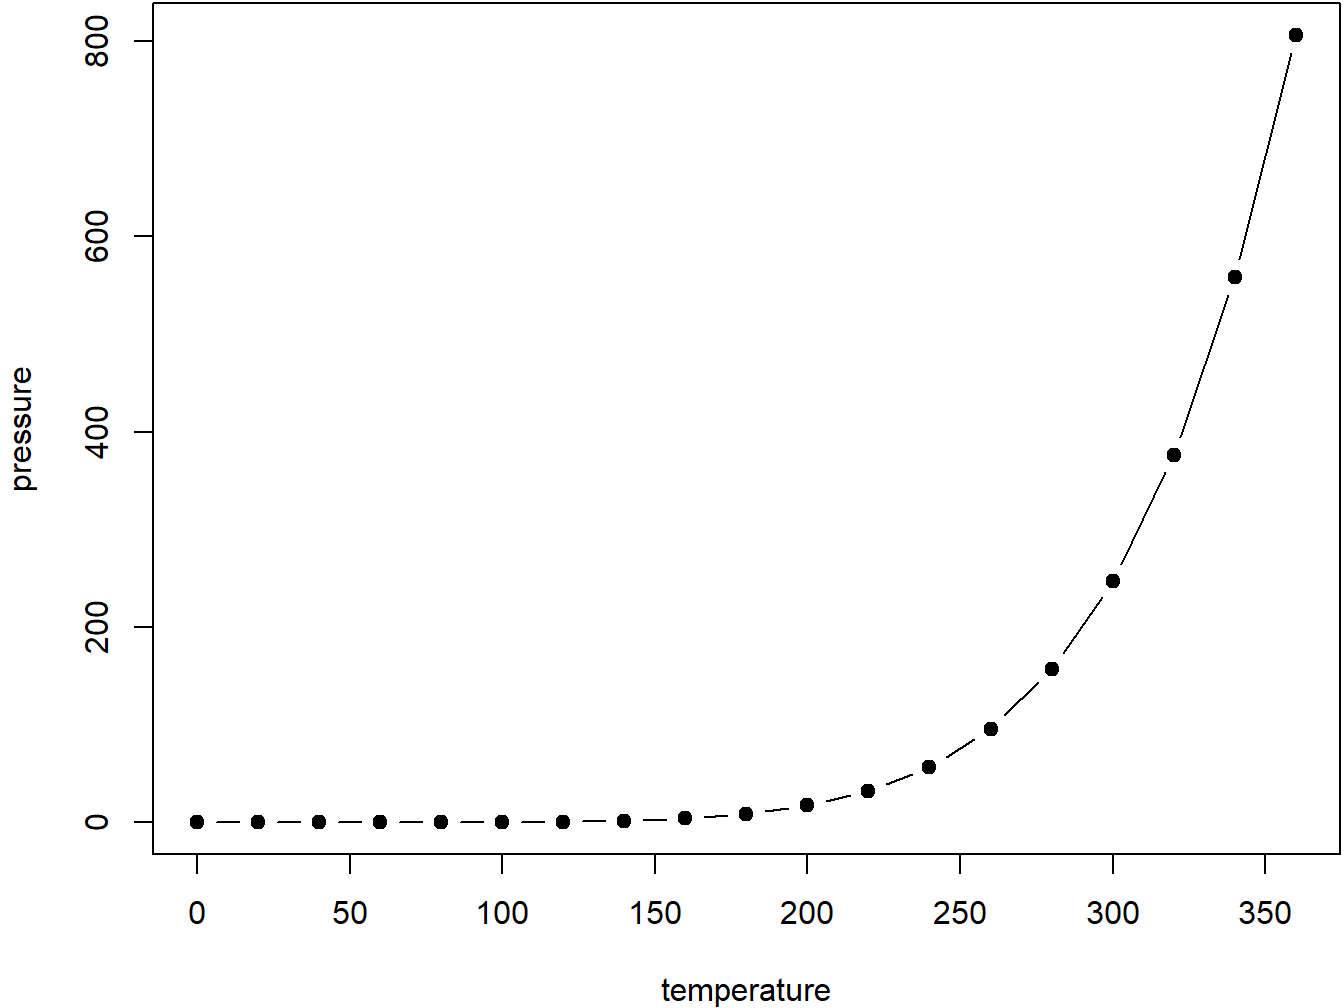
\includegraphics[width=0.8\linewidth]{Econ-2100-Coursepack_files/figure-latex/nice-fig-1} 

}

\caption{Here is a nice figure!}\label{fig:nice-fig}
\end{figure}

Don't miss Table \ref{tab:nice-tab}.

\begin{Shaded}
\begin{Highlighting}[]
\NormalTok{knitr}\SpecialCharTok{::}\FunctionTok{kable}\NormalTok{(}
  \FunctionTok{head}\NormalTok{(pressure, }\DecValTok{10}\NormalTok{), }\AttributeTok{caption =} \StringTok{\textquotesingle{}Here is a nice table!\textquotesingle{}}\NormalTok{,}
  \AttributeTok{booktabs =} \ConstantTok{TRUE}
\NormalTok{)}
\end{Highlighting}
\end{Shaded}

\begin{table}

\caption{\label{tab:nice-tab}Here is a nice table!}
\centering
\begin{tabular}[t]{rr}
\toprule
temperature & pressure\\
\midrule
0 & 0.0002\\
20 & 0.0012\\
40 & 0.0060\\
60 & 0.0300\\
80 & 0.0900\\
\addlinespace
100 & 0.2700\\
120 & 0.7500\\
140 & 1.8500\\
160 & 4.2000\\
180 & 8.8000\\
\bottomrule
\end{tabular}
\end{table}

\end{document}
